\begin{question}
Using the Euler scheme, write a program to simulate:
\begin{itemize}
\item a Wiener process;
\item a Brownian motion with $S_0 = 100$, $\mu=0.05$ and $\sigma=0.17$;
\item the stock price following a Geometric Brownian motion with $S_0 = 100$, $\mu=0.05$ and $\sigma=0.17$.
\end{itemize}
\end{question}

\cprotEnv\begin{solution}
\begin{ipython}
from numpy.random import normal, seed
import numpy as np

#initial price
S = 100
mu = 0.05
sigma = 0.17
T = 1 # total time
steps = 360 # 180 days simulation

seed(1)
wiener = [S]
abm = [S]
gbm = [S]

for i in range(steps):
    wiener.append(wiener[-1] + normal()*np.sqrt(T/steps))
    abm.append(abm[-1] + mu * T/steps + sigma * np.sqrt(T/steps) * normal())
    S = S * np.exp((mu - 0.5 * sigma * sigma) * T/steps + sigma * \
                    np.sqrt(T/steps) * normal())
    gbm.append(S)
\end{ipython}

\begin{figure}
\centering
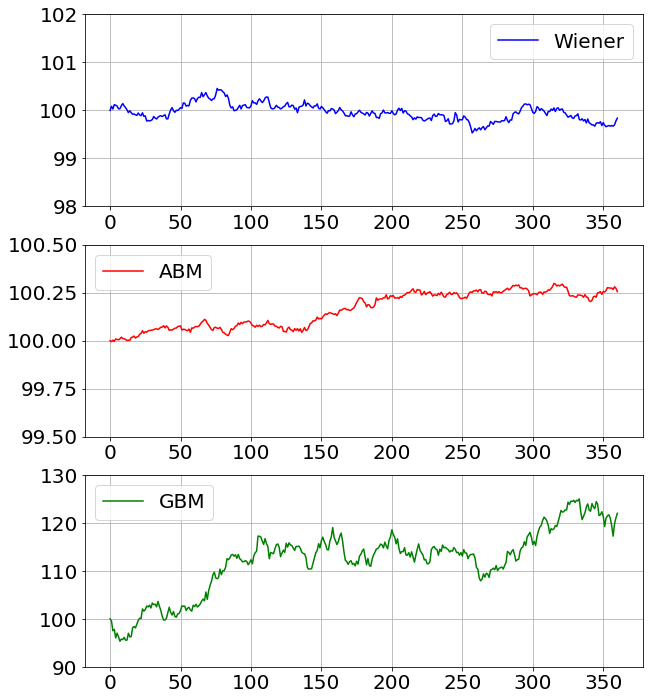
\includegraphics[width=0.7\linewidth]{figures/ex_stochastic}
\caption{Realizations of different kind of stochastic processes.}
\end{figure}
\end{solution}